\documentclass[]{tufte-handout}

% ams
\usepackage{amssymb,amsmath}

\usepackage{ifxetex,ifluatex}
\usepackage{fixltx2e} % provides \textsubscript
\ifnum 0\ifxetex 1\fi\ifluatex 1\fi=0 % if pdftex
  \usepackage[T1]{fontenc}
  \usepackage[utf8]{inputenc}
\else % if luatex or xelatex
  \makeatletter
  \@ifpackageloaded{fontspec}{}{\usepackage{fontspec}}
  \makeatother
  \defaultfontfeatures{Ligatures=TeX,Scale=MatchLowercase}
  \makeatletter
  \@ifpackageloaded{soul}{
     \renewcommand\allcapsspacing[1]{{\addfontfeature{LetterSpace=15}#1}}
     \renewcommand\smallcapsspacing[1]{{\addfontfeature{LetterSpace=10}#1}}
   }{}
  \makeatother

\fi

% graphix
\usepackage{graphicx}
\setkeys{Gin}{width=\linewidth,totalheight=\textheight,keepaspectratio}

% booktabs
\usepackage{booktabs}

% url
\usepackage{url}

% hyperref
\usepackage{hyperref}

% units.
\usepackage{units}


\setcounter{secnumdepth}{-1}

% citations
\usepackage{natbib}
\bibliographystyle{plainnat}


% pandoc syntax highlighting
\usepackage{color}
\usepackage{fancyvrb}
\newcommand{\VerbBar}{|}
\newcommand{\VERB}{\Verb[commandchars=\\\{\}]}
\DefineVerbatimEnvironment{Highlighting}{Verbatim}{commandchars=\\\{\}}
% Add ',fontsize=\small' for more characters per line
\newenvironment{Shaded}{}{}
\newcommand{\AlertTok}[1]{\textcolor[rgb]{1.00,0.00,0.00}{\textbf{#1}}}
\newcommand{\AnnotationTok}[1]{\textcolor[rgb]{0.38,0.63,0.69}{\textbf{\textit{#1}}}}
\newcommand{\AttributeTok}[1]{\textcolor[rgb]{0.49,0.56,0.16}{#1}}
\newcommand{\BaseNTok}[1]{\textcolor[rgb]{0.25,0.63,0.44}{#1}}
\newcommand{\BuiltInTok}[1]{\textcolor[rgb]{0.00,0.50,0.00}{#1}}
\newcommand{\CharTok}[1]{\textcolor[rgb]{0.25,0.44,0.63}{#1}}
\newcommand{\CommentTok}[1]{\textcolor[rgb]{0.38,0.63,0.69}{\textit{#1}}}
\newcommand{\CommentVarTok}[1]{\textcolor[rgb]{0.38,0.63,0.69}{\textbf{\textit{#1}}}}
\newcommand{\ConstantTok}[1]{\textcolor[rgb]{0.53,0.00,0.00}{#1}}
\newcommand{\ControlFlowTok}[1]{\textcolor[rgb]{0.00,0.44,0.13}{\textbf{#1}}}
\newcommand{\DataTypeTok}[1]{\textcolor[rgb]{0.56,0.13,0.00}{#1}}
\newcommand{\DecValTok}[1]{\textcolor[rgb]{0.25,0.63,0.44}{#1}}
\newcommand{\DocumentationTok}[1]{\textcolor[rgb]{0.73,0.13,0.13}{\textit{#1}}}
\newcommand{\ErrorTok}[1]{\textcolor[rgb]{1.00,0.00,0.00}{\textbf{#1}}}
\newcommand{\ExtensionTok}[1]{#1}
\newcommand{\FloatTok}[1]{\textcolor[rgb]{0.25,0.63,0.44}{#1}}
\newcommand{\FunctionTok}[1]{\textcolor[rgb]{0.02,0.16,0.49}{#1}}
\newcommand{\ImportTok}[1]{\textcolor[rgb]{0.00,0.50,0.00}{\textbf{#1}}}
\newcommand{\InformationTok}[1]{\textcolor[rgb]{0.38,0.63,0.69}{\textbf{\textit{#1}}}}
\newcommand{\KeywordTok}[1]{\textcolor[rgb]{0.00,0.44,0.13}{\textbf{#1}}}
\newcommand{\NormalTok}[1]{#1}
\newcommand{\OperatorTok}[1]{\textcolor[rgb]{0.40,0.40,0.40}{#1}}
\newcommand{\OtherTok}[1]{\textcolor[rgb]{0.00,0.44,0.13}{#1}}
\newcommand{\PreprocessorTok}[1]{\textcolor[rgb]{0.74,0.48,0.00}{#1}}
\newcommand{\RegionMarkerTok}[1]{#1}
\newcommand{\SpecialCharTok}[1]{\textcolor[rgb]{0.25,0.44,0.63}{#1}}
\newcommand{\SpecialStringTok}[1]{\textcolor[rgb]{0.73,0.40,0.53}{#1}}
\newcommand{\StringTok}[1]{\textcolor[rgb]{0.25,0.44,0.63}{#1}}
\newcommand{\VariableTok}[1]{\textcolor[rgb]{0.10,0.09,0.49}{#1}}
\newcommand{\VerbatimStringTok}[1]{\textcolor[rgb]{0.25,0.44,0.63}{#1}}
\newcommand{\WarningTok}[1]{\textcolor[rgb]{0.38,0.63,0.69}{\textbf{\textit{#1}}}}

% table with pandoc
\usepackage{longtable,booktabs,array}
\usepackage{calc} % for calculating minipage widths
% Correct order of tables after \paragraph or \subparagraph
\usepackage{etoolbox}
\makeatletter
\patchcmd\longtable{\par}{\if@noskipsec\mbox{}\fi\par}{}{}
\makeatother
% Allow footnotes in longtable head/foot
\IfFileExists{footnotehyper.sty}{\usepackage{footnotehyper}}{\usepackage{footnote}}
\makesavenoteenv{longtable}

% multiplecol
\usepackage{multicol}

% strikeout
\usepackage[normalem]{ulem}

% morefloats
\usepackage{morefloats}


% tightlist macro required by pandoc >= 1.14
\providecommand{\tightlist}{%
  \setlength{\itemsep}{0pt}\setlength{\parskip}{0pt}}

% title / author / date
\title[American Political Divides and Great Debates]{American Political
Divides and Great Debates}
\author{Prof.~Jonathan Cervas}
\date{Updated: August 25, 2025}


\begin{document}

\maketitle




\begin{quote}
Professor \textbf{Jonathan Cervas}\footnote{The most up-to-date version
  of this
  \href{https://github.com/jcervas/teaching/blob/main/2025-2026/class-cmu-84-309/syllabus.md}{syllabus
  can be found here}}\\
Office: Posner Hall 374\\
Email:
\textbf{\href{mailto:cervas@cmu.edu}{\nolinkurl{cervas@cmu.edu}}}\\
Location: POS 145 Time: Tuesday/Thursday 2:00p-3:20p Eastern Office
Hours: Wednesday 2-4p, and by appointment (arrange via email)\\
\href{https://www.cmu.edu/hub/calendar/}{\textbf{CMU Academic
Calendar}}\footnote{This course syllabus is a work in progress. The
  instructor will take note of student feedback and course schedule will
  evolve based on student preferences}
\end{quote}

\begin{quote}
TA: \textbf{Colleen Moosman}\\
Email:
\textbf{\href{mailto:cmoosman@andrew.cmu.edu}{\nolinkurl{cmoosman@andrew.cmu.edu}}}\\
Office Hours: Thursday 1:00p-2:00p
\end{quote}

\begin{quote}
\textbf{Course Relevance:} DC: Perspectives on Justice and Injustice\\
\textbf{Learning Resources:} All resources will be provided via Canvas\\
\textbf{Prerequisite Knowledge:} NONE
\end{quote}

\hypertarget{course-description}{%
\subsection{Course Description}\label{course-description}}

This course explores why Americans are so politically divided, how those
divisions create and reinforce inequalities, and what we can do to
address them. We look at key issues like voting rights, healthcare
access, racial and economic disparities, ethical uses of AI, and
environmental justice; though the topics will largely be selected by
students. Through discussions and debates, you will build critical
thinking, public speaking, and empathy skills. If you are interested in
political science, law, or social justice, this class will give you a
clear understanding of today's U.S. political landscape and ideas for
promoting fairness and equity at every level of society.

\hypertarget{learning-objectives}{%
\subsection{Learning Objectives}\label{learning-objectives}}

By the end of this course, students will be able to:

\begin{enumerate}
\def\labelenumi{\arabic{enumi}.}
\tightlist
\item
  \textbf{Explain} the historical and structural factors that contribute
  to political polarization in the United States.
\item
  \textbf{Describe} how political divisions intersect with and reinforce
  racial, economic, and social inequalities.
\item
  \textbf{Analyze} key policy issues (e.g., voting rights, healthcare,
  environmental justice) through the lens of fairness and equity.
\item
  \textbf{Evaluate} different perspectives on contentious political
  issues with empathy and critical reasoning.
\item
  \textbf{Apply} principles of ethical reasoning to assess the social
  impacts of emerging technologies such as artificial intelligence.
\item
  \textbf{Demonstrate} improved skills in public speaking, structured
  debate, and respectful civic discourse.
\item
  \textbf{Synthesize} information from political science, law, and
  social justice frameworks to form evidence-based arguments.
\item
  \textbf{Reflect} on their own values, biases, and roles as civic
  participants in a divided society.
\end{enumerate}

\hypertarget{grading}{%
\subsection{Grading}\label{grading}}

Your grade depends heavily on active engagement. This course is
interactive: your preparation (completing the readings), contributions
to discussions, and participation in debates are essential to your
success.

\emph{Assignments \& Deadlines} You are expected to meet all assignment
deadlines. If you anticipate being unable to turn something in on time,
contact me before the due date to discuss alternatives. Late work will
incur a small penalty\footnote{Typically one percentage point per day}
provided it does not impede your classmates' progress (for instance, in
group projects). Failing to participate or contribute meaningfully,
especially in ways that affect others' work, will result in a lower
grade.

\hypertarget{assessment}{%
\subsection{Assessment}\label{assessment}}

The course grade will be a weighted average of the following components:

\begin{longtable}[]{@{}
  >{\raggedright\arraybackslash}p{(\columnwidth - 2\tabcolsep) * \real{0.6667}}
  >{\raggedright\arraybackslash}p{(\columnwidth - 2\tabcolsep) * \real{0.3333}}@{}}
\toprule()
\begin{minipage}[b]{\linewidth}\raggedright
Assignment
\end{minipage} & \begin{minipage}[b]{\linewidth}\raggedright
Percent of Final Grade
\end{minipage} \\
\midrule()
\endhead
\textbf{Participation} & \textbf{25\%} \\
• \emph{Discussion \& In Class Assignments} & \emph{(5\%)} \\
• \emph{Attendance} & \emph{(15\%)} \\
• \emph{Student Led Topics} & \emph{(5\%)} \\
\textbf{Weekly Reflection Journals} & \textbf{15\%} \\
\textbf{Writing Modules} (3) & \textbf{3\%} \\
\textbf{Surveys} (2) & \textbf{2\%} \\
\textbf{Book Review} & \textbf{12\%} \\
• \emph{Written Review (3-5 single-spaced pages)} & \emph{(10\%)} \\
• \emph{In class Discussion} & \emph{(2\%)} \\
\textbf{Op-Ed Project} (Rough Draft + Final) & \textbf{20\%} \\
\textbf{AI-Powered Debate Simulation} (3) & \textbf{9\%} \\
\textbf{Final Capstone: Group Policy Brief} & \textbf{14\%} \\
\bottomrule()
\end{longtable}

\hypertarget{due-dates}{%
\subsection{Due Dates}\label{due-dates}}

\begin{longtable}[]{@{}ll@{}}
\toprule()
Assignment & Due Date \\
\midrule()
\endhead
Weekly Reflection Journals & Due Sundays, weekly \\
Writing Modules (3) & August 28, September 2, September 4 \\
Op-ed, first draft & September 22 \\
Op-ed peer review & September 25 \\
Op-ed final draft & September 29 \\
Book Review & October 13 \\
AI-Powered Debate Simulation & Weeks 4, 8, 10 \\
Group Project & December 2/4 \\
\bottomrule()
\end{longtable}

\hypertarget{assignment-details}{%
\subsection{Assignment Details}\label{assignment-details}}

\textbf{Participation \& Discussion} (25\%)

\emph{Purpose}: Civic discourse, empathy, critical thinking\\
\emph{Objective Alignment}: 4, 6, 8

\emph{Participation} (5\%): Active, respectful involvement in class
discussions, including preparedness (e.g., completing readings) and
thoughtful contributions.

\emph{Attendance} (15\%) Regular attendance and active involvement form
a significant part of your final grade (see grading section). If you do
not show up, you will not earn an `A'. To recognize that occasional
absences are sometimes unavoidable (e.g., for religious observance, job
interviews, university-sanctioned events, or illness), attendance grades
will be calculated using an exponential function. 1--2 absences → mild
penalty, 6+ absences → sharp drop (serious consequences).

\[s(A) = 100 \cdot \left(1 - \frac{1 - e^{-kA}}{1 - e^{-kT}} \right)\]
where \[k=0.1\] and \[A\] is the your number of absences and \[T\] is
the total number of classes.

\begin{figure}
\centering
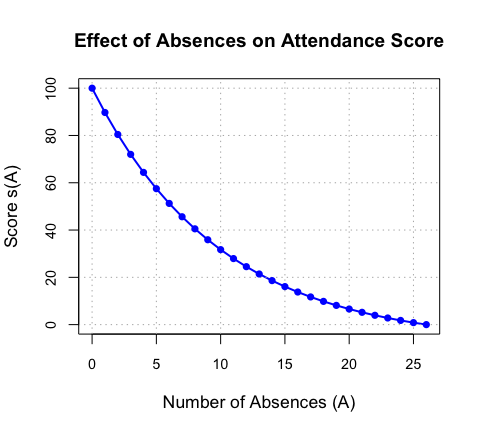
\includegraphics{readme_files/figure-gfm/attendance-curve-1.png}
\caption{Effect of Absences on Grade}
\end{figure}

If you must miss class, please notify me at least 24 hours in advance
(unless it is an emergency or sudden illness) so we can arrange a way
for you to catch up.\footnote{If you need to miss more than two sessions
  due to extenuating circumstances, let me know as soon as possible so
  we can discuss how best to support you.}

\emph{Student Led Topics} (5\%): Each student will lead one class
discussion on a topic of their choice related to the course themes
(along with several other students). This includes selecting readings,
preparing discussion questions, and facilitating the conversation. The
goal is to engage your peers in critical thinking and respectful debate.
Topics and readings should be assigned early in the semester.

\textbf{Weekly Reflection Journals} (15\%)

\emph{Purpose}: Personal reflection, connection to course theme\\
\emph{Objective Alignment}: 1, 2, 4, 8

\begin{itemize}
\tightlist
\item
  Short (300-500 word) reflections on how class topics connect to
  current events, reactions to course readings, or evolving viewpoints.
\item
  Graded as complete/incomplete based on effort and engagement.
\end{itemize}

\textbf{Writing Modules} (3\%)

\emph{Purpose}: Language (vocabulary, tone, social conventions) is
appropriate and aligned to audience's needs. Evidence (types, placement,
volume, specificity) is appropriate and aligned to audience's needs\\
\emph{Objective Alignment}: 1, 3, 5\\
Not grade for completion, but for effort and engagement.

\begin{itemize}
\tightlist
\item
  Students complete 1 module per day (may not complete all at once).
  Canvas will make activity 2 and 3 available 24 hours after a student
  completes previous activity
\item
  Module 1: Adapting Writing for a New Audience
\item
  Module 2: Creating an Audience Profile
\item
  Module 3: Revising Writing to provide audience-focused feedback
\end{itemize}

\textbf{Book Review Assignment} (12\%)

\emph{Purpose}: Deep analysis, critical evaluation, communication\\
\emph{Objective Alignment}: 1, 2, 3, 4, 6, 7

\begin{itemize}
\tightlist
\item
  \textbf{Written Review} (10\%)
\end{itemize}

\emph{Purpose}: Argument analysis, assumption critique, implication
discussion

\begin{itemize}
\tightlist
\item
  \emph{Length}: 3-5 single-spaced pages (approx. 1,500--2,500 words)
\item
  \emph{Content Guidelines}:

  \begin{itemize}
  \tightlist
  \item
    Summarize the author's central argument(s) succinctly.
  \item
    Critically evaluate those arguments using logical reasoning and
    textual evidence.
  \item
    Identify any assumptions or ideological lenses the author brings.
  \item
    Discuss broader political, ethical, or social implications.
  \item
    Make connections to course themes such as inequality, polarization,
    or justice.
  \item
    Use citations for any quoted or paraphrased material.
  \end{itemize}
\item
  \textbf{In class Discussion} (2\%)
\end{itemize}

\emph{Purpose}: Verbal synthesis, peer engagement, clarity of thought\\
\emph{Format}: Small Group Discussions

\begin{itemize}
\tightlist
\item
  \emph{Expectations}:

  \begin{itemize}
  \tightlist
  \item
    Clear, engaging summary of key ideas from the book.
  \item
    Highlight your critical take or most interesting insight.
  \item
    Encourage discussion by posing a question or provocation.
  \end{itemize}
\end{itemize}

\textbf{Op-ed w/ peer-review} (20\%)

\emph{Purpose}: Persuasive writing, revision, public engagement\\
\emph{Objective Alignment}: 1, 2, 3, 5, 7

\begin{itemize}
\tightlist
\item
  Drawing on a topic related to this course, or something political from
  your own life or experience, write an op-ed that could be published in
  a newspaper or blog.
\item
  \textbf{Rough Draft} (2\%) \& \textbf{Peer Review} (8\%)

  \begin{itemize}
  \tightlist
  \item
    \emph{Length}: There is a strict 1,250-word limit.
  \item
    \emph{Content Guidelines}:

    \begin{itemize}
    \tightlist
    \item
      Prepare a short essay advocating for (or against) any social or
      political issue of your choosing (topics relating to American
      politics).
    \item
      The idea is that you will write something that can be submitted to
      a newspaper or internet blog.
    \item
      Concise arguments made for a more general audience are the goal of
      this assignment; something your parents can read and understand.
    \item
      The use of data and visualizations is strongly encouraged and is
      not included in the word count.
    \end{itemize}
  \item
    Peer review should address the substance of the paper, along with
    grammar (e.g., ``Is the thesis clear?'', ``Is evidence
    convincing?'', ``Does it speak to a broader audience?'').

    \begin{itemize}
    \tightlist
    \item
      You will complete peer reviews of two classmate's drafts,
      providing constructive feedback on clarity, argument strength, and
      engagement.
    \end{itemize}
  \end{itemize}
\item
  \textbf{Final Draft} (10\%)

  \begin{itemize}
  \tightlist
  \item
    Using the feedback from your peers, revise your op-ed to improve
    clarity, argumentation, and engagement.
  \end{itemize}
\end{itemize}

\textbf{AI-Powered Debate Simulation} (10\%)

\emph{Purpose}: Perspective-taking, applied argumentation, tech-enhanced
learning\\
\emph{Objective Alignment}: 4, 5, 6, 8

\begin{itemize}
\tightlist
\item
  \emph{Description}: Students interact with or program AI-generated
  personas (e.g., a libertarian voter, environmental activist, rural
  health worker) to simulate debates on divisive policy topics.
\item
  \emph{Options}: Use tools like ChatGPT to role-play or build simple
  scripted bots that represent different ideological views.
\item
  \emph{Goal}: Understand ideological nuance and test one's arguments
  against realistic opposition.
\item
  \emph{Deliverables}: Transcript
\end{itemize}

\textbf{Final Capstone: Group Policy Brief} (30\%)

\emph{Purpose}: Research, equity-centered solutions, teamwork
\emph{Objective Alignment}: 3, 5, 7

\begin{itemize}
\tightlist
\item
  \textbf{Written Brief}: Small teams choose a politically polarizing
  issue tied to inequality (e.g., gerrymandering, Medicaid expansion,
  tech bias) and write a formal policy brief
  (\textasciitilde1,500--2,000 words).

  \begin{itemize}
  \tightlist
  \item
    \emph{Components}:

    \begin{itemize}
    \tightlist
    \item
      Executive Summary
    \item
      Problem Definition
    \item
      Background/Context
    \item
      Policy Options \& Stakeholder Analysis
    \item
      Recommendation(s)
    \item
      Equity Impact Statement
    \end{itemize}
  \end{itemize}
\item
  \textbf{Presentation}: Teams present findings in a mock legislative or
  community forum during finals week.
\end{itemize}

\begin{center}\rule{0.5\linewidth}{0.5pt}\end{center}

\begin{Shaded}
\begin{Highlighting}[]
\CommentTok{\# \# Readings to add}
\CommentTok{\# {-} \_Optional\_: “Power, Performance, and Legitimacy.” Journal of Democracy. https://www.journalofdemocracy.org/articles/power{-}performance{-}and{-}legitimacy/}
\CommentTok{\# {-} Kleinfeld, R. (2023). Polarization, Democracy, and Political Violence in the United States: What the Research Says. Carnegie Endowment for International Peace.}
\CommentTok{\#     * [https://carnegieendowment.org/research/2023/09/polarization{-}democracy{-}and{-}political{-}violence{-}in{-}the{-}united{-}states{-}what{-}the{-}research{-}says?lang=en](https://carnegieendowment.org/research/2023/09/polarization{-}democracy{-}and{-}political{-}violence{-}in{-}the{-}united{-}states{-}what{-}the{-}research{-}says?lang=en)}
\end{Highlighting}
\end{Shaded}

\hypertarget{course-schedule-subject-to-change-as-semester-progresses}{%
\section{Course Schedule (Subject to Change as Semester
Progresses):}\label{course-schedule-subject-to-change-as-semester-progresses}}

\hypertarget{august-26-syllabus-day}{%
\subsection{August 26: Syllabus Day}\label{august-26-syllabus-day}}

\begin{itemize}
\tightlist
\item
  \textbf{Introduction to the Course}; topic selection, draft
  privacy/free speech statement

  \begin{itemize}
  \tightlist
  \item
    Lewsey, Story: Fred. 2020. ``Faith in democracy: millennials are the
    most disillusioned generation `in living memory.'\,''
    \url{https://www.cam.ac.uk/stories/youthanddemocracy}
  \end{itemize}
\end{itemize}

\hypertarget{august-28}{%
\subsection{August 28}\label{august-28}}

\textbf{The Fence}

\begin{itemize}
\tightlist
\item
  Background on ``The Fence''

  \begin{itemize}
  \tightlist
  \item
    \url{https://www.cmu.edu/stugov/fence/index.html}
  \end{itemize}
\item
  President Farnam's Statement about the Fence after Trump Visit

  \begin{itemize}
  \tightlist
  \item
    \href{https://view.connect.cmu.edu/?qs=9827695e1300b223c66dc479ff67774b2636d3862de5ba00c9a33d4302a496ddcaf11df3a82f9e278459b95e9d5ee66d1142ed95ebf2e444469cb9e124411e4d6f6a1f56aec0be5427e909c8e70b5fdc}{Statement
    1}
  \item
    \href{https://view.connect.cmu.edu/?qs=d5ffef9eec97a8068120b2ae007393146e19f012eb1422f95848b0a34d534b2e1f9f223a78511d4e3a52621e5d0aa96979ac815d57172df6e4829d10878251adfa53d1d6402581641ffd4f9ec001f75b}{Statement
    2}
  \end{itemize}
\item
  Articles from \emph{The Tartan} about The Fence`s history

  \begin{itemize}
  \tightlist
  \item
    \url{https://github.com/jcervas/teaching/blob/main/2025-2026/class-cmu-2025-84-309/readings/The-True-History-of-the-Fence-I.md}\strut \\
  \item
    \url{https://github.com/jcervas/teaching/blob/main/2025-2026/class-cmu-2025-84-309/readings/The-True-History-of-the-Fence-II.md}
  \item
    \url{https://github.com/jcervas/teaching/blob/main/2025-2026/class-cmu-2025-84-309/readings/The-True-History-of-the-Fence-III.md}
  \end{itemize}
\end{itemize}

\hypertarget{september-2}{%
\subsection{September 2}\label{september-2}}

\textbf{America's Founding: Enlightened or Enslaved?}

\begin{enumerate}
\def\labelenumi{\arabic{enumi}.}
\tightlist
\item
  \_*The 1619 Project\_
\end{enumerate}

\begin{itemize}
\tightlist
\item
  ``America Wasn't a Democracy Until Black Americans Made It One'' --
  Essay by Nikole Hannah-Jones
  \url{https://www.nytimes.com/interactive/2019/08/14/magazine/black-history-american-democracy.html}

  \begin{itemize}
  \tightlist
  \item
    Introduces the central thesis of the project: re-centering slavery
    and Black Americans in the nation's founding narrative.
  \end{itemize}
\item
  ``In Order to Understand the Brutality of American Capitalism, You
  Have to Start on the Plantation'' -- Essay by Matthew Desmond
  \url{https://www.nytimes.com/interactive/2019/08/14/magazine/slavery-capitalism.html}

  \begin{itemize}
  \tightlist
  \item
    Connects slavery to contemporary economic systems.
  \end{itemize}
\end{itemize}

\begin{enumerate}
\def\labelenumi{\arabic{enumi}.}
\setcounter{enumi}{1}
\tightlist
\item
  \emph{The 1776 Report}
\end{enumerate}

--
\href{https://trumpwhitehouse.archives.gov/wp-content/uploads/2021/01/The-Presidents-Advisory-1776-Commission-Final-Report.pdf}{Arnn,
Larry P., Carol Swain, and Matthew Spalding. 2021. The President's
Advisory 1776 Commission. Washington, D.C: The White House.} - Presents
a traditionalist, patriotic framing of American founding values.

\hypertarget{september-4}{%
\subsection{September 4}\label{september-4}}

\begin{enumerate}
\def\labelenumi{\arabic{enumi}.}
\tightlist
\item
  \emph{The 1776 Report}
\end{enumerate}

\begin{itemize}
\tightlist
\item
  ``AHA Statement Condemning Report of Advisory 1776 Commission.''

  \begin{itemize}
  \tightlist
  \item
    \url{https://www.historians.org/news/aha-statement-condemning-report-of-advisory-1776-commission/}
  \end{itemize}
\item
  McKenna, Konstantin. 2025. ``The 1776 Project Is a Desperate Search
  for the Right Enemies.'' Foreign Policy.

  \begin{itemize}
  \tightlist
  \item
    \url{https://foreignpolicy.com/2021/01/21/1776-project-desperate-search-enemies-identity-politics-unamerican/}
  \end{itemize}
\end{itemize}

\begin{enumerate}
\def\labelenumi{\arabic{enumi}.}
\setcounter{enumi}{1}
\tightlist
\item
  \emph{The 1619 Project}
\end{enumerate}

\begin{itemize}
\tightlist
\item
  Hannah-Jones, Nikole. 2019. The 1619 Project. The New York Times
  Magazine.

  \begin{itemize}
  \tightlist
  \item
    \href{https://pulitzercenter.org/sites/default/files/full_issue_of_the_1619_project.pdf?_gl=1*av7vjw*_gcl_au*MTA2MTEwMzQ4NS4xNzUwODgxODA1*_ga*MjA3ODQ2OTEyMi4xNzUwODgxODA1*_ga_ZYQYTZTT61*czE3NTA4ODE4MDMkbzEkZzEkdDE3NTA4ODI2NzEkajM4JGwwJGgxNjcwMTY0ODcx}{https://pulitzercenter.org/sites/default/files/full\_issue\_of\_the\_1619\_project.pdf?\_gl=1\emph{av7vjw}\_gcl\_au\emph{MTA2MTEwMzQ4NS4xNzUwODgxODA1}\_ga\emph{MjA3ODQ2OTEyMi4xNzUwODgxODA1}\_ga\_ZYQYTZTT61*czE3NTA4ODE4MDMkbzEkZzEkdDE3NTA4ODI2NzEkajM4JGwwJGgxNjcwMTY0ODcx}
  \end{itemize}
\item
  Silverstein, Jake. 2020. ``On Recent Criticism of The 1619 Project.''
  The New York Times.

  \begin{itemize}
  \tightlist
  \item
    \url{https://www.nytimes.com/2020/10/16/magazine/criticism-1619-project.html}
  \end{itemize}
\item
  ``We Respond to the Historians Who Critiqued The 1619 Project.'' 2019.
  The New York Times.

  \begin{itemize}
  \tightlist
  \item
    \url{https://www.nytimes.com/2019/12/20/magazine/we-respond-to-the-historians-who-critiqued-the-1619-project.html}
  \end{itemize}
\end{itemize}

\begin{enumerate}
\def\labelenumi{\arabic{enumi}.}
\setcounter{enumi}{2}
\tightlist
\item
  \textbf{Optional for ambitious students}
\end{enumerate}

\begin{itemize}
\tightlist
\item
  Frederick Douglass, ``What to the Slave is the Fourth of July?''
  (1852)

  \begin{itemize}
  \tightlist
  \item
    (\textasciitilde20 min read, historical context for both projects)
  \end{itemize}
\end{itemize}

\hypertarget{september-9}{%
\subsection{September 9}\label{september-9}}

\textbf{Free Speech in Schools}

\begin{itemize}
\item
  Chemerinsky, Erwin. 2024. ``The Underlying Issues Concerning Free
  Speech in Schools.'' Stanford Law Review 76: 1427.
\item
  \url{https://www.stanfordlawreview.org/print/article/the-underlying-issues-concerning-free-speech-in-schools/}
\item
  Chemerinsky, Erwin, and Howard Gillman. 2018. Free speech on campus.
  Paperback edition. New Haven\,; London: Yale University Press.

  \begin{itemize}
  \tightlist
  \item
    Chapter 1: The New Censorship
  \item
    Chapter 2: Why Is Free Speech Important?
  \end{itemize}
\end{itemize}

\hypertarget{september-11}{%
\subsection{September 11}\label{september-11}}

\begin{itemize}
\tightlist
\item
  Chemerinsky, Erwin, and Howard Gillman. 2018. Free speech on campus.
  Paperback edition. New Haven\,; London: Yale University Press.

  \begin{itemize}
  \tightlist
  \item
    Chapter 3: Nullius in Verba: Free Speech at Colleges and
    Universities
  \item
    Chapter 4: Hate Speech
  \end{itemize}
\end{itemize}

\hypertarget{september-16}{%
\subsection{September 16}\label{september-16}}

\begin{itemize}
\tightlist
\item
  Chemerinsky, Erwin, and Howard Gillman. 2018. Free speech on campus.
  Paperback edition. New Haven\,; London: Yale University Press.
\item
  Chapter 5: What Campuses Can and Can't Do
\item
  Chapter 6: What's at Stake?
\end{itemize}

\hypertarget{september-18}{%
\subsection{September 18}\label{september-18}}

\begin{itemize}
\tightlist
\item
  Iyengar, Shanto. 2025. ``Identity Politics, Party Polarization, and
  the Rise of Donald Trump.'' In The Changing Character of the American
  Right, Volume I: Ideology, Politics and Policy in the Era of Trump,
  eds.~Joel D. Aberbach et al.~Cham: Springer Nature Switzerland,
  p.~79--94.

  \begin{itemize}
  \tightlist
  \item
    \url{https://doi.org/10.1007/978-3-031-73168-6_4}
  \end{itemize}
\end{itemize}

\hypertarget{september-23}{%
\subsection{September 23}\label{september-23}}

\textbf{Racism in Policing}

\emph{Guest Lecture}: Ralph L. Bangs

\emph{Former Associate Director, Center on Race and Social Problems,
School of Social Work, University of Pittsburgh}

\begin{itemize}
\tightlist
\item
  ``Pittsburgh's Massive Racial Disparities in Police Actions,
  2021-2023'' July 1, 2024.

  \begin{itemize}
  \tightlist
  \item
    \href{https://www.canva.com/design/DAGQTToI1A0/q3ld4QrnSxyaBG8aMxJIRQ/view?utm_content=DAGQTToI1A0\&utm_campaign=designshare\&utm_medium=link\&utm_source=editor}{Op-Ed
    Link:
    https://www.canva.com/design/DAGQTToI1A0/q3ld4QrnSxyaBG8aMxJIRQ/view?utm\_content=DAGQTToI1A0\&utm\_campaign=designshare\&utm\_medium=link\&utm\_source=editor}
  \end{itemize}
\item
  ``Police Discrimination Against Black Youth Under Age 18'' October 1,
  2024.

  \begin{itemize}
  \tightlist
  \item
    \href{https://www.canva.com/design/DAGSX13mhds/KJRJOKXLUTgJiJTZqrWk3Q/view?utm_content=DAGSX13mhds\&utm_campaign=designshare\&utm_medium=link\&utm_source=editor}{Op-Ed
    Link:
    https://www.canva.com/design/DAGSX13mhds/KJRJOKXLUTgJiJTZqrWk3Q/view?utm\_content=DAGSX13mhds\&utm\_campaign=designshare\&utm\_medium=link\&utm\_source=editor}
  \end{itemize}
\end{itemize}

Optional: - Bangs, R. ``Fourth Amendment Problems with Pittsburgh Police
Policies'' February 2025 *
\url{https://www.crsp.pitt.edu/fourth-amendment-problems-pittsburgh-police-policies}
- Bangs, R. ``Pittsburgh Leaders Must Recognize the Serious Racial
Problems in Police Actions'' January 2025 *
\url{https://live-racesocialproblems-pitt.pantheonsite.io/pittsburgh-leaders-must-recognize-serious-racial-problems-police-actions}
- Bangs, R. ``Racial Disparities and Discrimination in Drug Arrest
Charges by Pittsburgh Police, January-October 2022'' November 2024 *
\url{https://www.crsp.pitt.edu/racial-disparities-and-discrimination-drug-arrest-charges-pittsburgh-police-january-october-2022}
- Bangs, R. ``New National Reports on Anti-Black Pretextual Traffic
Stops and Frisks, Related Pittsburgh Police Data, and Recommendations''
October 15, 2024 *
\url{https://www.crsp.pitt.edu/new-national-reports-anti-black-pretextual-traffic-stops-and-frisks-related-pittsburgh-police-data}

\hypertarget{september-25}{%
\subsection{September 25}\label{september-25}}

\begin{itemize}
\tightlist
\item
  Klein, Ezra. 2020. Why We're Polarized. Avid Reader Press / Simon \&
  Schuster.

  \begin{itemize}
  \tightlist
  \item
    \url{https://books.google.com/books?id=1G6gDwAAQBAJ}
  \end{itemize}
\item
  Klein, Introduction: What Didn't Happen
\item
  Klein, Chapter 1: How Democrats Became Liberals and Republicans Became
  Conservatives
\end{itemize}

\hypertarget{september-30}{%
\subsection{September 30}\label{september-30}}

\begin{itemize}
\tightlist
\item
  Klein, Chapter 2: The Dixiecrat Dilemma
\item
  Klein, Chapter 3: Your Brain on Groups
\end{itemize}

\hypertarget{october-2}{%
\subsection{October 2}\label{october-2}}

\textbf{The Internet and Social Media}

\begin{itemize}
\tightlist
\item
  Larreguy, Horacio, and Pia J. Raffler. 2025. ``Accountability in
  Developing Democracies: The Impact of the Internet, Social Media, and
  Polarization.'' Annual Review of Political Science 28(Volume 28,
  2025): 413--434.

  \begin{itemize}
  \tightlist
  \item
    \url{https://www.annualreviews.org/content/journals/10.1146/annurev-polisci-033123-015559}
  \end{itemize}
\item
  Barrett, Paul, Justin Hendrix, and Grant Sims. 2021. Fueling the Fire:
  How Social Media Intensifies U.S. Political Polarization And What Can
  Be Done About It. NYU Stern Center for Business and Human Rights.

  \begin{itemize}
  \tightlist
  \item
    \url{https://bhr.stern.nyu.edu/wp-content/uploads/2024/02/NYUCBHRFuelingTheFire_FINALONLINEREVISEDSep7.pdf}
  \end{itemize}
\item
  Shapiro, Ari. 2022. ``How the polarizing effect of social media is
  speeding up.'' NPR.

  \begin{itemize}
  \tightlist
  \item
    \url{https://www.npr.org/2022/09/09/1121295499/facebook-twitter-youtube-instagram-tiktok-social-media}
  \end{itemize}
\end{itemize}

\hypertarget{october-7}{%
\subsection{October 7}\label{october-7}}

\textbf{Mid-Semester FEC } with Eberly Center (Patrick Walsh)
\textbf{Guest, Jonathan Lai, Politico}

Read his \href{https://www.politico.com/staff/jonathan-lai}{bio here}.

\begin{itemize}
\tightlist
\item
  Topic and readings TBA

  \begin{itemize}
  \tightlist
  \item
    (Public Funding of News)
  \item
    (distinguishing between ``democracy'' and ``America'')
  \end{itemize}
\end{itemize}

\hypertarget{october-9}{%
\subsection{October 9}\label{october-9}}

\textbf{Guest, Jonathan Lai, Politico}

Topic and readings TBA

\hypertarget{october-14}{%
\subsection{October 14}\label{october-14}}

\textbf{FALL BREAK}, no class

\hypertarget{october-16}{%
\subsection{October 16}\label{october-16}}

\textbf{FALL BREAK}, no class

\hypertarget{october-21}{%
\subsection{October 21}\label{october-21}}

\begin{itemize}
\tightlist
\item
  Klein, Chapter 4: The Press Secretary in Your Mind
\item
  Klein, Chapter 5: Demographic Threat
\end{itemize}

\hypertarget{october-23}{%
\subsection{October 23,}\label{october-23}}

\begin{itemize}
\tightlist
\item
  Klein, Chapter 6: The Media Divide beyond Left-Right
\item
  Klein, Chapter 7: Post-Persuasion Elections
\end{itemize}

\hypertarget{october-28}{%
\subsection{October 28,}\label{october-28}}

\begin{itemize}
\tightlist
\item
  Klein, Chapter 8: When Bipartisanship Becomes Irrational
\item
  Klein, Chapter 9: The Difference between Democrats and Republicans
\item
  Klein, Chapter 10: Managing Polarization---and Ourselves
\end{itemize}

\hypertarget{october-30}{%
\subsection{October 30}\label{october-30}}

Student led topics/debates

\hypertarget{november-4}{%
\subsection{November 4}\label{november-4}}

DEMOCRACY DAY, no class
\href{https://www.cmu.edu/student-affairs/slice/civic-engagement/advocacy/voter/index.html}{\textbf{Register
to Vote}}

\emph{Join us for CMU's third Democracy Day, an opportunity to focus on
our institutional commitment to civic service and democracy on Election
Day. There will be programming and resources available throughout the
day for our entire community to engage on the key ideals of democracy.}

\emph{There are no classes on Democracy Day prior to 5 p.m. and the
entire CMU community ---faculty, staff and students --- is encouraged to
participate as their schedules allow.}

\hypertarget{november-6}{%
\subsection{November 6}\label{november-6}}

Student led topics/debates

\hypertarget{november-11}{%
\subsection{November 11}\label{november-11}}

Student led topics/debates

\hypertarget{november-13}{%
\subsection{November 13}\label{november-13}}

Student led topics/debates

\hypertarget{november-18}{%
\subsection{November 18}\label{november-18}}

Student led topics/debates

\hypertarget{november-20}{%
\subsection{November 20}\label{november-20}}

Student led topics/debates

\hypertarget{november-25}{%
\subsection{November 25}\label{november-25}}

No class because many people will be missing.

\hypertarget{november-27}{%
\subsection{November 27}\label{november-27}}

\textbf{THANKSGIVING DAY}, no class

\hypertarget{december-2}{%
\subsection{December 2}\label{december-2}}

Group Policy Brief

\hypertarget{december-4}{%
\subsection{December 4}\label{december-4}}

Group Policy Brief

\begin{center}\rule{0.5\linewidth}{0.5pt}\end{center}

\hypertarget{potential-topics-for-student-led-discussions}{%
\subsection{Potential topics for Student Led
Discussions}\label{potential-topics-for-student-led-discussions}}

\textbf{Immigration Politics}

\begin{itemize}
\tightlist
\item
  \url{https://www.whitehouse.gov/presidential-actions/2025/01/protecting-the-american-people-against-invasion/}
\item
  \url{https://www.cfr.org/backgrounder/us-immigration-debate-0}
\end{itemize}

\textbf{Affirmative Action} (STUDENTS FOR FAIR ADMISSIONS, INC. v.
PRESIDENT AND FELLOWS OF HARVARD COLLEGE, No.~20--1199)) - Decided June
29, 2023

\begin{itemize}
\tightlist
\item
  Opinion of the Court

  \begin{itemize}
  \tightlist
  \item
    ROBERTS, C. J., delivered the opinion of the Court, in which THOMAS,
    ALITO, GORSUCH, KAVANAUGH, and BARRETT, JJ., joined.

    \begin{itemize}
    \tightlist
    \item
      \url{https://www.supremecourt.gov/opinions/22pdf/20-1199_hgdj.pdf}
    \end{itemize}
  \end{itemize}
\item
  Dissent

  \begin{itemize}
  \tightlist
  \item
    SOTOMAYOR, J., filed a dissenting opinion, in which KAGAN, J.,
    joined, and in which JACKSON, J., joined as it applies to
    No.~21--707.
  \end{itemize}
\item
  Concurring \& other Dissenting Opinions

  \begin{itemize}
  \tightlist
  \item
    THOMAS, J., filed a concurring opinion.
  \item
    GORSUCH, J., filed a concurring opinion, in which THOMAS, J.,
    joined.
  \item
    KAVANAUGH, J., filed a concurring opinion.
  \item
    JACKSON, J., filed a dissenting opinion in No.~21--707, in which
    SOTOMAYOR and KAGAN, JJ., joined.
  \end{itemize}
\end{itemize}

\textbf{Birthright Citizenship}

\textbf{Regulating AI}

\begin{center}\rule{0.5\linewidth}{0.5pt}\end{center}

\hypertarget{student-privacy-in-class-discussions}{%
\subsection{Student Privacy in Class
Discussions}\label{student-privacy-in-class-discussions}}

Students to draft this provision in week 1.

\begin{center}\rule{0.5\linewidth}{0.5pt}\end{center}

\hypertarget{course-principles}{%
\subsection{Course Principles}\label{course-principles}}

Throughout this course, we will engage with several key themes that
intersect and build upon one another to deepen our understanding of the
complex social and political landscape in the United States.
Conversations should be open, free, and respectful.

\begin{enumerate}
\def\labelenumi{\arabic{enumi}.}
\item
  \textbf{Analyzing a Range of Perspectives and Political Divides}\\
  One of our primary themes is exploring how different communities'
  experiences shape political divides. We will critically examine how
  underrepresented voices---those with distinct histories, challenges,
  and worldviews---contribute to a growing political polarization.
  Understanding these varied experiences is essential for grasping the
  roots of political conflict and for developing strategies that bridge
  divides.
\item
  \textbf{The Significance of Varied Viewpoints in Justice and
  Injustice}\\
  We will delve into why recognizing and valuing multiple perspectives
  is crucial for identifying instances of injustice that might otherwise
  be overlooked. By centering viewpoints from communities whose
  experiences differ from the majority, we gain insight into how justice
  is perceived, enacted, and sometimes denied. This work will guide us
  toward more equitable approaches to social and political challenges.
\item
  \textbf{The Role of Systems and Institutions in Perpetuating
  Inequality}\\
  Another critical theme is examining how U.S. institutions and systems
  have historically reinforced privilege and power imbalances. We will
  analyze how laws, policies, and institutional practices shape access
  to resources, opportunities, and rights---often disadvantaging certain
  groups. By understanding these systemic forces, we can begin to
  address the root causes of injustice.
\item
  \textbf{Ethical Obligations to Address Inequality}\\
  Throughout the semester, we will reflect on our individual and
  collective responsibility to confront inequalities. This includes
  considering how we can uplift underrepresented voices, advocate for
  fair policies, and work against oppressive structures. These
  reflections will encourage us to think critically about our roles in
  society and the impact of our actions on the broader pursuit of
  justice.
\end{enumerate}

\begin{quote}
\emph{These themes will be woven into our discussions, readings, and
assignments. By the end of the semester, you will have developed a
nuanced perspective on how identity, power, and politics intersect---and
you'll be equipped to contribute to meaningful change in your
communities.}
\end{quote}

\hypertarget{ai-use-policy-for-student-work}{%
\subsection{AI Use Policy for Student
Work}\label{ai-use-policy-for-student-work}}

As artificial intelligence (AI) tools become increasingly accessible, it
is important to clarify expectations for their use in this course. You
are welcome to use AI technologies (such as ChatGPT, Grammarly, or
similar tools) to support your independent work---such as brainstorming
ideas, checking grammar, or improving the clarity of your writing.
However, you \textbf{may not use AI to generate substantive content that
you submit as your own original work}. All assignments, essays, and
projects must reflect your own analysis, critical thinking, and voice.

\textbf{Permitted Uses of AI:}

\begin{itemize}
\tightlist
\item
  Outlining or organizing your thoughts
\item
  Checking grammar, spelling, or clarity
\item
  Generating ideas or prompts to help you get started
\item
  Reviewing your own drafts for readability
\end{itemize}

\textbf{Prohibited Uses of AI:}

\begin{itemize}
\tightlist
\item
  Submitting AI-generated essays, paragraphs, or answers as your own
  work
\item
  Using AI to complete assignments, discussion posts, or projects in
  place of your own effort
\item
  Copying and pasting AI-generated content without substantial revision
  and personal input
\end{itemize}

If you use AI tools in your process, you must \textbf{disclose} how you
used them in a brief note at the end of your assignment (e.g., ``I used
ChatGPT to help brainstorm ideas for my outline.'').

\textbf{Violations:}\\
Submitting AI-generated content as your own is considered academic
dishonesty and will be treated as a violation of the university's
academic integrity policy.

If you have questions about what is or is not allowed, please ask before
submitting your work.

\begin{center}\rule{0.5\linewidth}{0.5pt}\end{center}

\hypertarget{representation-statement}{%
\subsection{Representation Statement}\label{representation-statement}}

I am committed to including a broad range of perspectives in the
readings and materials for this course. If you believe a critical voice
is missing, please let me know so I can improve the syllabus now and in
future offerings.

\textbf{We must treat every individual with respect.} We come from many
different backgrounds, and this variety of viewpoints is fundamental to
building and maintaining an equitable and inclusive campus community.
``Representation'' can refer to the ways we identify ourselves---race,
color, national origin, language, sex, disability, age, sexual
orientation, gender identity, religion, creed, ancestry, belief, veteran
status, or genetic information, among others. Each of these identities
shapes the perspectives our students, faculty, and staff bring to
campus. Promoting these varied viewpoints not only fuels excellence and
innovation but also advances the pursuit of justice. We acknowledge our
imperfections while fully committing to the work---inside and outside
our classrooms---of building and sustaining a campus community that
embraces these core values.

Each of us is responsible for creating a safer, more inclusive
environment.

Unfortunately, incidents of bias or discrimination do occur, whether
intentional or unintentional. They contribute to an unwelcoming
atmosphere for individuals and groups at the university. Therefore, the
university encourages anyone who experiences or observes unfair or
hostile treatment on the basis of identity to speak out for justice and
seek support---either in the moment or afterward. You can share your
experiences using the following resources:

\begin{itemize}
\tightlist
\item
  \textbf{Ethics Reporting Hotline}\\
  Submit an anonymous report by calling 844-587-0793 or visiting
  \textbf{cmu.ethicspoint.com}.\\
  All reports are documented and reviewed to determine whether further
  action is needed. Regardless of the incident type, the university will
  use your feedback to transform our campus climate into one that is
  more equitable and just.
\end{itemize}

\begin{center}\rule{0.5\linewidth}{0.5pt}\end{center}

\hypertarget{accommodations-for-students-with-disabilities}{%
\subsection{Accommodations for Students with
Disabilities}\label{accommodations-for-students-with-disabilities}}

If you have a documented disability and an accommodations letter from
the Office of Disability Resources, please discuss your needs with me as
early in the semester as possible. I will work with you to ensure that
accommodations are provided as appropriate. If you suspect you may have
a disability and are not yet registered with the Office of Disability
Resources, you can contact them at
\textbf{\href{mailto:access@andrew.cmu.edu}{\nolinkurl{access@andrew.cmu.edu}}}.

\begin{center}\rule{0.5\linewidth}{0.5pt}\end{center}

\hypertarget{student-well-being}{%
\subsection{Student Well-Being}\label{student-well-being}}

The past few years have been challenging. We are all under significant
stress and uncertainty. I encourage you to find ways to move regularly,
eat well, and reach out to your support system---or to me at
\textbf{\href{mailto:cervas@cmu.edu}{\nolinkurl{cervas@cmu.edu}}}---if
you need help. We can all benefit from support during stressful times,
and this semester is no exception.

As a student, you may experience a range of challenges that interfere
with learning, such as strained relationships, increased anxiety,
substance use, feeling down, difficulty concentrating, or lack of
motivation. These mental health concerns or stressful events can
diminish your academic performance and reduce your ability to
participate in daily activities. CMU offers services that can help, and
treatment does work. Learn more about confidential mental health
services available on campus at:

\begin{itemize}
\tightlist
\item
  \textbf{Counseling and Psychological Services}:
  \url{http://www.cmu.edu/counseling/}\\
  Phone (24/7): 412-268-2922
\end{itemize}

Please remember that support is always available---don't hesitate to
reach out.

\begin{center}\rule{0.5\linewidth}{0.5pt}\end{center}

\hypertarget{eberly-center}{%
\subsection{Eberly Center}\label{eberly-center}}

Students,

This semester, I am working with the Eberly Center on educational
research. Because of this, I have included a statement about the
research and your rights as a research participant in your syllabus.
That same statement along with common questions can be found below in
this email.

Please reach out to Laura Pottmeyer
\href{mailto:lpottmey@andrew.cmu.edu}{\nolinkurl{lpottmey@andrew.cmu.edu}}
with any questions about the study.

Best,

Jonathan

\begin{center}\rule{0.5\linewidth}{0.5pt}\end{center}

\textbf{Research to Improve the Course}

For this class, the Eberly Center is working with your instructor on
educational research. This research will involve your coursework. You
will not be asked to do anything above and beyond the normal learning
activities and assignments that are part of this course. You are free
not to participate in this research, and your participation will have no
influence on your grade for this course or your academic career at CMU.
If you do not wish to participate or if you are under 18 years of age,
please send an email to Laura Pottmeyer
(\href{mailto:lpottmey@andrew.cmu.edu}{\nolinkurl{lpottmey@andrew.cmu.edu}}),
and then your data will not be included. Participants will not receive
any compensation. The data collected as part of this research will
include student grades. All analyses of data from participants'
coursework will be conducted after the course is over and final grades
are submitted. In the future, once we have removed all identifiable
information from your data, we may use the data for our future research
studies, or we may distribute the data to other researchers for their
research studies. The Eberly Center will conduct the data analysis and
interpretation of the results for this research project. The Eberly
Center for Teaching Excellence \& Educational Innovation is located on
the CMU-Pittsburgh Campus and its mission is to support the professional
development of all CMU instructors regarding teaching and learning. To
minimize the risk of breach of confidentiality, the Eberly Center will
never have access to data from this course containing your personal
identifiers. All data will be analyzed in de-identified form and
presented in the aggregate, without any personal identifiers. If you
have questions pertaining to your rights as a research participant, or
to report concerns to this study, please contact Laura Pottmeyer
(\href{mailto:lpottmey@andrew.cmu.edu}{\nolinkurl{lpottmey@andrew.cmu.edu}}).

\begin{center}\rule{0.5\linewidth}{0.5pt}\end{center}

\textbf{Plain language interpretation}:

\begin{itemize}
\tightlist
\item
  After the semester is over, the data generated by students in this
  course, which often comes from things like assignments, projects,
  surveys, etc., is stripped of all identifying information and
  aggregated into a larger research dataset for analysis.
\item
  As a potential participant in this research, you have a say in what
  happens to your data. If you are OK with data generated by you in this
  course being de-identified and aggregated into a larger research
  dataset, then there is nothing you need to do - simply proceed through
  the course as you would with any other course.
\item
  IF you would NOT like your data to be used for that purpose (or you
  are under 18) that is when you email Laura Pottmeyer and say ``Hi
  Laura, this is my name and course number, I would like to opt-out,
  thanks, goodbye'', and your data will not be included in the research
  analyses.
\item
  This opt-out process is confidential, and your instructors will not
  know whether you have opted out or not.
\item
  Importantly, your decision in this matter will NOT affect your
  experience in the course. You are only making a decision about what
  happens to your data AFTER the course is over.
\end{itemize}

Below are some potential questions students may have\ldots{}

\begin{longtable}[]{@{}
  >{\raggedright\arraybackslash}p{(\columnwidth - 2\tabcolsep) * \real{0.2126}}
  >{\raggedright\arraybackslash}p{(\columnwidth - 2\tabcolsep) * \real{0.7874}}@{}}
\toprule()
\begin{minipage}[b]{\linewidth}\raggedright
\textbf{QUESTION}
\end{minipage} & \begin{minipage}[b]{\linewidth}\raggedright
\textbf{ANSWER}
\end{minipage} \\
\midrule()
\endhead
What do I need to do? & If you would like to opt out of your data being
used in research analyses, all you need to do is email Laura Pottmeyer
(email is in the syllabus) with your name, course number, and say ``I'd
like to opt out''. \textbf{If you do not wish to opt out, you do not
need to do anything}. \\
What is this research about? & Unfortunately, we cannot provide further
details at this time. If, after the course is over, you are curious
about this kind of work, please feel free to contact Laura Pottmeyer or
anyone else at the Eberly Center
(\href{mailto:lpottmey@andrew.cmu.edu}{\nolinkurl{lpottmey@andrew.cmu.edu}}). \\
Do I have to make up my mind right now? & No, there is no need to make
up your mind right now. You can choose to opt out anytime, even if it is
on the last day of the semester. \\
What if I don't want to participate? & If you'd like to opt out, the
only thing that will change is what happens to your data AFTER the
course is over. \textbf{Your required coursework will be the same
regardless of your decision}. \\
Can I see the results? & Often the results from this kind of work do not
come together right away. If you are curious about the results after
this course is over, please feel free to contact Laura Pottmeyer, and we
would be happy to give you an update, if possible. \\
How will the data be used? & In two ways: to help improve the course and
to contribute to educational research on how students learn best. Note
that all analyses occur after course grades are submitted and student
identifiers are removed. \\
If I opt out, do I still have to complete work assigned by the
instructor? & Yes. \\
\bottomrule()
\end{longtable}

\bibliography{bib.bib}



\end{document}
